\documentclass[tikz,border=1cm]{standalone}
\usetikzlibrary{calc,angles}
\begin{document}
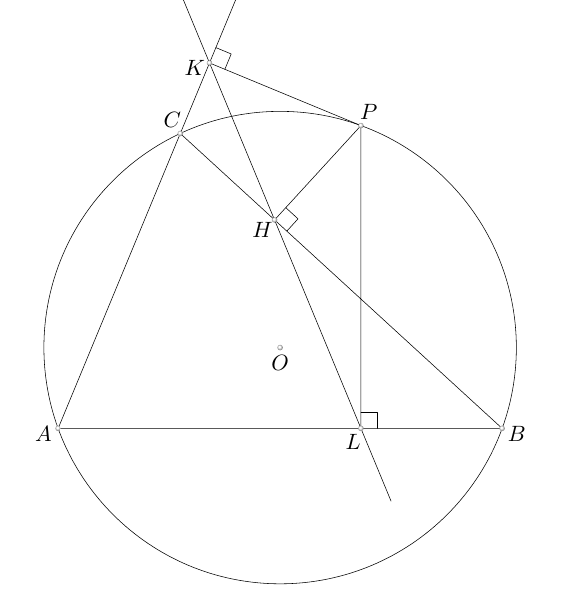
\begin{tikzpicture}[very thin,join=round,cap=round,declare function={r=3;}]
    \path(0:0)coordinate(O)(200:r)coordinate(A)(-20:r)coordinate(B)(115:r)coordinate(C)(70:r)coordinate(P) ($(B)!(P)!(C)$)coordinate(H) ($(A)!(P)!(C)$)coordinate(K) ($(B)!(P)!(A)$)coordinate(L)
    ($(C)!1.5!(K)$)coordinate(C');
    \draw(O)circle(r);
    \draw(A)--(B)--(C)--cycle (K)--(P)--(H)(P)--(L);
    \draw[shorten >=-1cm,shorten <=-1cm](K)--(L);
    \draw[shorten >=-1cm](C)--(K);
    \pic[draw,angle radius=6]{right angle=B--L--P};
    \pic[draw,angle radius=6]{right angle=B--H--P};
    \pic[draw,angle radius=6]{right angle=P--K--C'};
    \foreach \p/\g in{O/-90,A/-160,B/-20,C/120,P/60,H/-140,K/-160,L/-120}\shade[ball color=white](\p)circle(1pt)node[shift={(\g:.2)},scale=.8]{$\p$};
\end{tikzpicture}

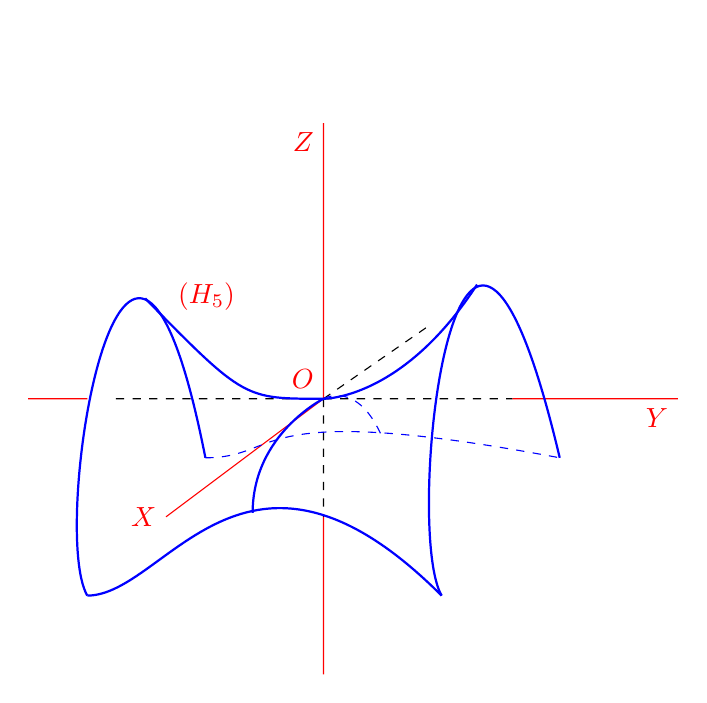
\begin{tikzpicture}[join=round]
    \def\a{1.5}
    \def\h{2.5}
    \draw[red] (0,0)--(0,3.5) node[below left]{$Z$} (0,-0.6*\h)--(0,-3.5) (1.6*\a,0)--(4.5,0) node[below left]{$Y$} (0,0)--(-2,-1.5) node[left]{$X$} (0,0) node[above left]{$O$} (-1,1.3) node[left]{$(H_{5})$} (-2.5*\a,0)--(-2*\a,0);
    \draw[dashed] (0,0)--(1.6*\a,0) (0,0)--(0,-0.6*\h) (0,0)--(-1.8*\a,0) (0,0)--(1.3,0.9);
    \draw[blue,thick] (\a,-\h)..controls +(120:1) and (70:5)..(2*\a,-0.3*\h);
    \draw[blue,thick] (-0.6*\a,-0.58*\h)..controls +(90:1) and (90:0)..(0,0);
    \draw[blue,dashed] (0,0)..controls +(-90:0) and (30:0.5)..(0.5*\a,-0.2*\h);
    \draw[blue,thick] (0,0)..controls +(0:0) and (-1:1)..(1.3*\a,0.58*\h);
    \draw[blue,thick] (-2*\a,-\h)..controls +(120:1) and (120:5)..(-\a,-0.3*\h);
    \draw[blue,thick] (0,0)..controls +(0:-1) and (1:-1)..(-1.51*\a,0.51*\h);
    \draw[blue,thick] (-2*\a,-\h)..controls +(0:1) and (0:-1)..(\a,-\h);
    \draw[blue,dashed] (-\a,-0.3*\h)..controls +(0:1) and (0:-1)..(2*\a,-0.3*\h);
\end{tikzpicture}


\end{document}